% Options for packages loaded elsewhere
\PassOptionsToPackage{unicode}{hyperref}
\PassOptionsToPackage{hyphens}{url}
\PassOptionsToPackage{dvipsnames,svgnames,x11names}{xcolor}
%
\documentclass[
  11pt,
]{article}
\usepackage{amsmath,amssymb}
\usepackage{iftex}
\ifPDFTeX
  \usepackage[T1]{fontenc}
  \usepackage[utf8]{inputenc}
  \usepackage{textcomp} % provide euro and other symbols
\else % if luatex or xetex
  \usepackage{unicode-math} % this also loads fontspec
  \defaultfontfeatures{Scale=MatchLowercase}
  \defaultfontfeatures[\rmfamily]{Ligatures=TeX,Scale=1}
\fi
\usepackage{lmodern}
\ifPDFTeX\else
  % xetex/luatex font selection
\fi
% Use upquote if available, for straight quotes in verbatim environments
\IfFileExists{upquote.sty}{\usepackage{upquote}}{}
\IfFileExists{microtype.sty}{% use microtype if available
  \usepackage[]{microtype}
  \UseMicrotypeSet[protrusion]{basicmath} % disable protrusion for tt fonts
}{}
\makeatletter
\@ifundefined{KOMAClassName}{% if non-KOMA class
  \IfFileExists{parskip.sty}{%
    \usepackage{parskip}
  }{% else
    \setlength{\parindent}{0pt}
    \setlength{\parskip}{6pt plus 2pt minus 1pt}}
}{% if KOMA class
  \KOMAoptions{parskip=half}}
\makeatother
\usepackage{xcolor}
\usepackage[margin=1in]{geometry}
\usepackage{longtable,booktabs,array}
\usepackage{calc} % for calculating minipage widths
% Correct order of tables after \paragraph or \subparagraph
\usepackage{etoolbox}
\makeatletter
\patchcmd\longtable{\par}{\if@noskipsec\mbox{}\fi\par}{}{}
\makeatother
% Allow footnotes in longtable head/foot
\IfFileExists{footnotehyper.sty}{\usepackage{footnotehyper}}{\usepackage{footnote}}
\makesavenoteenv{longtable}
\usepackage{graphicx}
\makeatletter
\def\maxwidth{\ifdim\Gin@nat@width>\linewidth\linewidth\else\Gin@nat@width\fi}
\def\maxheight{\ifdim\Gin@nat@height>\textheight\textheight\else\Gin@nat@height\fi}
\makeatother
% Scale images if necessary, so that they will not overflow the page
% margins by default, and it is still possible to overwrite the defaults
% using explicit options in \includegraphics[width, height, ...]{}
\setkeys{Gin}{width=\maxwidth,height=\maxheight,keepaspectratio}
% Set default figure placement to htbp
\makeatletter
\def\fps@figure{htbp}
\makeatother
\setlength{\emergencystretch}{3em} % prevent overfull lines
\providecommand{\tightlist}{%
  \setlength{\itemsep}{0pt}\setlength{\parskip}{0pt}}
\setcounter{secnumdepth}{-\maxdimen} % remove section numbering
\usepackage{mathptmx}\usepackage{caption}\captionsetup{font=small}\usepackage{xurl}\sloppy\AtBeginEnvironment{longtable}{\footnotesize}
\ifLuaTeX
  \usepackage{selnolig}  % disable illegal ligatures
\fi
\IfFileExists{bookmark.sty}{\usepackage{bookmark}}{\usepackage{hyperref}}
\IfFileExists{xurl.sty}{\usepackage{xurl}}{} % add URL line breaks if available
\urlstyle{same}
\hypersetup{
  pdftitle={When AI Risk Benchmarks Fail to Transfer to Life or Death Stakes},
  pdfauthor={John Blakeslee {[}affiliation{]}},
  colorlinks=true,
  linkcolor={violet},
  filecolor={Maroon},
  citecolor={Blue},
  urlcolor={violet},
  pdfcreator={LaTeX via pandoc}}

\title{When AI Risk Benchmarks Fail to Transfer to Life or Death Stakes}
\usepackage{etoolbox}
\makeatletter
\providecommand{\subtitle}[1]{% add subtitle to \maketitle
  \apptocmd{\@title}{\par {\large #1 \par}}{}{}
}
\makeatother
\subtitle{Whether a language model's risk attitude on lotteries predicts
its advice when lives are at stake depends on how the model is run}
\author{John Blakeslee {[}affiliation{]}}
\date{Full draft, November 14 2026. For Phil Armour and the TNL
residency. Not for circulation.}

\begin{document}
\maketitle

\emph{Draft status.} Every section is written. The numbers come from
data already in the repository, and no new model runs were made for this
draft. Open-model numbers are from \texttt{analysis/stage\_a.py} and
\texttt{analysis/stage\_a\_bounds.py} (Stage A, on main). Frontier
numbers are from \texttt{analysis/paper\_frontier\_tables.py}, written
for this draft, which pools the self and advise roles and resamples
gambles for the 95\% intervals, and from
\texttt{docs/frontier-results-2026-10-20.md}. Figures 2 to 4 are made by
\texttt{analysis/make\_frontier\_figures.py}. Items in {[}square
brackets{]} are to do before arXiv.

\hypertarget{abstract}{%
\subsection{Abstract}\label{abstract}}

Language models are increasingly consulted as advisers on consequential
decisions, including in defense and crisis response, and their attitude
to risk is usually measured with lotteries over money. We ask whether
that measurement predicts their advice when lives are at stake. We
restate 40 money gambles, number for number, as decisions about
civilians evacuated, soldiers brought out and detained aid workers
freed. Each is posed as the model's own decision and as a recommendation
to an official, in gain and loss wording, with each option listed first.
On three open 7-8B models the shift is large. Qwen2.5-7B is 0.27 to 0.64
less likely to take the gamble with lives than with money, and when it
reasons first its money answers explain at most a quarter of the
question-to-question variation in its lives answers. On four Claude
models the result depends on how the model is run. In snap answers and
with written reasoning, every model is far more cautious with lives
(Claude Sonnet 5.5 is 0.23 to 0.63 less likely to take the gamble), and
money answers predict lives answers poorly. With extended thinking
switched on, Claude Haiku 5.5 and Claude Opus 5.5 choose by expected
value in every domain and money predicts lives well (r about 0.9), even
though they think for only 55 to 90 tokens. Within Claude Sonnet 5.5 and
Claude Fable 5.1 the effort setting acts like a dose. At high effort
their caution with civilians and soldiers falls by half or more, while
their caution about detained aid workers holds at every setting, in a
second wording, and when we remove the escalation clause the models cite
as their reason. A lottery can screen advisory risk only for some models
in some modes, and an evaluator learns which only by running the
advisory questions. Risk evaluations for advisory use should therefore
be run on advisory questions at the inference setting used in
deployment, and should report that setting the way a clinical trial
reports a dose.

\hypertarget{introduction}{%
\subsection{1. Introduction}\label{introduction}}

Nobody deploys a language model to choose lotteries. It is deployed to
advise. An analyst asks which course of action to brief, a staff officer
asks for a recommendation, and an official asks whether to press for
more or take what is on the table. Defense and intelligence users are
adopting language models for analysis, planning support and wargaming,
and many of the decisions involved share a familiar structure, in which
a sure, moderate outcome is weighed against a gamble with a larger
upside and a real chance of losing everything.

The standard way to learn how a model handles that trade-off borrows
from experimental economics. The evaluator offers the model a series of
choices between a sure amount of money and a gamble, and reads off its
risk attitude (Holt and Laury 2002; Chen et al.~2023; Liu et al. 2025;
Wang et al.~2025). The measurement is cheap, repeatable and comparable
across models. If it predicts the model's advice, it is a ready-made
screening test for advisory deployments. If it does not, evaluations
have to be run on the advisory task itself.

We test the link directly. We take 40 money gambles from an instrument
we had already validated on the same open models and restate each one,
with the same numbers, as a choice about people. The three settings are
evacuating civilians from a besieged city, withdrawing soldiers from an
isolated position, and negotiating the release of detained aid workers.
Each question is posed both as the model's own decision and as a
recommendation to a civilian official, a combatant commander or a senior
negotiator, in gain and loss wording, with each option listed first.
Free-outcome controls offer two sure amounts and check that the model
prefers more people saved to fewer. We run the grid on three open
models, where we can read choice probabilities exactly, and on four
Claude models through the provider's API. The Claude models answer in
three modes, namely a one-letter snap answer, written reasoning before
the answer, and the provider's extended thinking at several effort
settings.

We report five findings.

\begin{enumerate}
\def\labelenumi{\arabic{enumi}.}
\tightlist
\item
  With lives at stake, the models become much more cautious, and the
  money answers do not predict by how much. Qwen2.5-7B, reasoning first,
  takes the gamble in 81\% of money questions where the gamble pays
  more, and in 17\% (civilians), 32\% (soldiers) and 18\% (detained aid
  workers) of the matching lives questions. Its reasoning states a
  preference for certainty. Claude Sonnet 5.5 in snap answers takes the
  money gamble almost every time and is 0.23 to 0.63 less likely to take
  it with lives.
\item
  Snap advice on lives can be set by the format of the question.
  Llama-3.1-8B's one-letter answers in every lives domain follow
  whichever option is listed first. Sonnet's snap answers on civilians
  and soldiers swing by 0.40 to 0.46 with option order, against almost
  nothing for money.
\item
  Extended thinking can close the gap, and the length of the reasoning
  does not explain it. With extended thinking on, Claude Haiku 5.5 and
  Claude Opus 5.5 choose by expected value in every domain (agreement
  0.94 to 1.00), and their money answers predict their lives answers
  with r of about 0.9. They think for 55 to 90 tokens. Haiku's written
  reasoning is nearly three times as long and leaves the gap in place.
\item
  Within one model, the effort setting acts like a dose. For Sonnet and
  Fable, raising effort from low to high cuts the caution with civilians
  and soldiers by half or more, while thinking grows only from about 70
  to 90 tokens (Sonnet) or from 34 to 79 (Fable).
\item
  In two of the four Claude models, caution about detained people
  survives every setting. Sonnet and Fable remain 0.29 to 0.47 less
  likely to gamble for detainees than for money at every effort, in a
  second wording, and when the escalation clause is removed, even though
  Sonnet's written reasoning cites escalation in every detainee answer.
\end{enumerate}

The results support a conditional version of the claim we set out to
test. A money lottery screens a model's advisory risk posture well for
some models in some modes and badly for others, and nothing in the
lottery itself tells the evaluator which case applies. The thinking
setting is part of what is being evaluated.

Section 2 places the work in the literature and section 3 describes the
design. Section 4 reports the open models, section 5 the Claude models
in their three modes, section 6 the effort results, and section 7 the
detainee exception. Section 8 uses the project's earlier results on the
same instrument to explain why lottery answers transfer poorly. Section
9 sets out what the results mean for evaluating models meant to advise,
section 10 lists limitations, and section 11 concludes.

\hypertarget{related-work}{%
\subsection{2. Related work}\label{related-work}}

\hypertarget{risk-and-framing-in-language-models}{%
\subsubsection{Risk and framing in language
models}\label{risk-and-framing-in-language-models}}

A growing literature reads economic preferences off language models with
the tools of experimental economics, including choices over lotteries,
framing manipulations and structural estimation (Binz and Schulz 2023;
Chen et al.~2023; Horton 2023; Mei et al.~2024; Liu et al. 2025; Wang et
al.~2025; Bini et al.~2026). Instruction tuning has been linked to
human-like cognitive biases such as framing effects (Itzhak et
al.~2024), and more capable models have been found to drop intuitive
biases and behave ``hyperrationally'' (Hagendorff, Fabi and Kosinski
2023). This project's earlier phases measured risk curvature, loss
aversion and framing on the same 40 gambles across base and post-trained
models. Nearly all of this work measures preferences over money. Mazeika
et al.~(2025) elicit utilities over outcomes that include lives and find
they grow more coherent with scale, and Trhlik et al.~(2026) show that
such measured values shift with the deployment context. We are not aware
of work that gives a model the same lotteries in money and in lives,
number for number, and asks whether one predicts the other.

\hypertarget{framing-and-risk-over-lives-in-people}{%
\subsubsection{Framing and risk over lives in
people}\label{framing-and-risk-over-lives-in-people}}

Our lives domains are a structured version of Tversky and Kahneman's
(1981) disease problem. People are more risk averse and more sensitive
to framing with lives than with money (Fagley and Miller 1997).
Dual-process accounts of moral judgment hold that controlled reasoning
favors the outcome-maximizing option while intuition resists it (Greene
et al.~2001, 2008). Many outcome-maximizing responses turn out to be
intuitive, though (Bago and De Neys 2019), and more thought does not
reliably reduce framing effects in people (LeBoeuf and Shafir 2003).
People also hold some values as protected. They refuse to trade such
values against quantities and condemn even considering the trade (Baron
and Spranca 1997; Tetlock et al.~2000; Tetlock 2003). Each of these
strands bears on one of our results.

\hypertarget{reasoning-and-moral-choice-in-language-models}{%
\subsubsection{Reasoning and moral choice in language
models}\label{reasoning-and-moral-choice-in-language-models}}

Pfeffer, Krügel and Uhl (2025) report that reasoning models give more
utilitarian answers to trolley-style dilemmas, and Himmelreich (2026)
finds that much of that difference reflects prompt confounds and
refusals. Samway et al.~(2025) find that chain-of-thought traces lean
deontological while after-the-fact explanations lean consequentialist.
Cheung, Maier and Lieder (2025) find stronger omission bias in language
models than in people. Hosseini, Khanna and Pierce (2026) report that
model choices diverge further from human ones as reasoning ability
rises, and more test-time compute does not always improve answers (Gema
et al.~2025). Most of this work compares reasoning and non-reasoning
models, which confounds the model with the mode. We vary the mode and
the effort setting within the same model, on matched questions with no
refusals.

\hypertarget{language-models-in-military-and-crisis-decisions}{%
\subsubsection{Language models in military and crisis
decisions}\label{language-models-in-military-and-crisis-decisions}}

Rivera et al.~(2024) ran language-model agents as nations in a wargame
and found escalation in all five models they studied, including
arms-race dynamics and, rarely, nuclear use. Lamparth et al.~(2024)
compared models with 107 national-security experts in a US-China crisis
wargame and found the models could be more aggressive and more sensitive
to scenario changes than human teams. Both studies observe behavior in
rich scenarios. Neither measures an underlying risk attitude and asks
whether it explains the behavior. Our structured lives questions find
caution instead. Alongside those studies, this suggests that a model's
risk posture depends on the domain and on the format of the question.

\hypertarget{evaluation-validity}{%
\subsubsection{Evaluation validity}\label{evaluation-validity}}

Benchmark scores are often read as measuring general capacities they
were not built to measure (Raji et al.~2021). For values and opinions in
particular, constrained multiple-choice answers can fail to predict what
the same model says in open-ended use (Röttger et al.~2024). Our
question is the risk-preference version of this concern. We ask whether
a cheap, standard measurement carries over to the use that matters.

\hypertarget{design}{%
\subsection{3. Design}\label{design}}

\hypertarget{gambles-domains-roles-and-frames}{%
\subsubsection{Gambles, domains, roles and
frames}\label{gambles-domains-roles-and-frames}}

The gambles are the 40 items of instrument 2 from Phase 3 of this
project. Each sets a sure amount against a single-prize gamble, with
probabilities and payoffs chosen so that expected values straddle the
sure amount (expected-value ratios from about 0.5 to 2). Payoffs are
non-round and the wording is novel, to limit contamination.

Across domains the numbers stay fixed and only the units change, as the
table below shows.

\begin{longtable}[]{@{}
  >{\raggedright\arraybackslash}p{(\columnwidth - 6\tabcolsep) * \real{0.2500}}
  >{\raggedright\arraybackslash}p{(\columnwidth - 6\tabcolsep) * \real{0.2500}}
  >{\raggedright\arraybackslash}p{(\columnwidth - 6\tabcolsep) * \real{0.2500}}
  >{\raggedright\arraybackslash}p{(\columnwidth - 6\tabcolsep) * \real{0.2500}}@{}}
\toprule\noalign{}
\begin{minipage}[b]{\linewidth}\raggedright
Domain
\end{minipage} & \begin{minipage}[b]{\linewidth}\raggedright
Sure option
\end{minipage} & \begin{minipage}[b]{\linewidth}\raggedright
Risky option
\end{minipage} & \begin{minipage}[b]{\linewidth}\raggedright
Failure branch
\end{minipage} \\
\midrule\noalign{}
\endhead
\bottomrule\noalign{}
\endlastfoot
Money & gain \$s for certain & p chance of \$h & nothing \\
Civilians & evacuate s civilians for certain & p chance to evacuate h &
none evacuated \\
Troops & bring s soldiers out for certain & p chance to bring h out &
none come out \\
Detainees & accept a deal freeing s & press for full release, p chance h
freed & talks collapse, the crisis escalates, none freed \\
\end{longtable}

In the self role the model decides (``You command an isolated
unit\ldots{}''). In the advise role it recommends (``A combatant
commander with an isolated unit asks you to recommend\ldots{}''). The
gain frame starts from nothing and offers a sure amount against a chance
at the prize. The mixed frame starts with the sure amount in hand and
offers to keep it or take a chance of rising to the prize or falling to
zero. The two frames describe the same choice over final outcomes.

\hypertarget{order-controls-and-grid-size}{%
\subsubsection{Order, controls and grid
size}\label{order-controls-and-grid-size}}

Every question appears with each option first. Ten free-outcome controls
per domain and role offer two sure amounts, and a model that engages
with the question picks the larger. The full grid is 4 domains x 2 roles
x (40 gambles x 2 frames x 2 orders + 10 controls x 2 orders), or 1,440
questions. The reasoning and thinking runs use the 20 gambles of the
Phase 3 reasoning runs, or 800 questions.

\hypertarget{second-wording-and-the-release-variant-stage-a2}{%
\subsubsection{Second wording and the release variant (Stage
A2)}\label{second-wording-and-the-release-variant-stage-a2}}

To separate the domain from the template, every domain also has a
second, independently written wording. A fifth domain, ``release'',
repeats the original detainee wording with the escalation clause
deleted, so that the failure branch reads ``talks collapse and none are
freed''. It tests whether the threat of escalation drives caution in
that domain, as opposed to the people at stake. Stage A2 has 1,800 snap
questions and 1,000 reasoning or thinking questions, and was run on the
Claude models only.

\hypertarget{open-models}{%
\subsubsection{Open models}\label{open-models}}

Qwen2.5-7B-Instruct and Llama-3.1-8B-Instruct are prompted in chat
format and OLMo-2-1124-7B-Instruct few-shot. We read each from its
next-token probabilities on A and B, which gives P(risky) exactly. Each
model answers in two regimes, an immediate one-letter answer and greedy
reasoning followed by the answer.

\hypertarget{claude-models}{%
\subsubsection{Claude models}\label{claude-models}}

We ran Claude Haiku 5.5, Claude Sonnet 5.5, Claude Opus 5.5 and Claude
Fable 5.1 through the native Anthropic API at the default temperature in
October 2026. Each question is sampled several times (five for snap
answers, three otherwise), and P(risky) is the share of answers that
pick the gamble. The models answer in up to three modes.

\begin{longtable}[]{@{}
  >{\raggedright\arraybackslash}p{(\columnwidth - 4\tabcolsep) * \real{0.3333}}
  >{\raggedright\arraybackslash}p{(\columnwidth - 4\tabcolsep) * \real{0.3333}}
  >{\raggedright\arraybackslash}p{(\columnwidth - 4\tabcolsep) * \real{0.3333}}@{}}
\toprule\noalign{}
\begin{minipage}[b]{\linewidth}\raggedright
Mode
\end{minipage} & \begin{minipage}[b]{\linewidth}\raggedright
What the model does
\end{minipage} & \begin{minipage}[b]{\linewidth}\raggedright
Open-model counterpart
\end{minipage} \\
\midrule\noalign{}
\endhead
\bottomrule\noalign{}
\endlastfoot
Snap & Extended thinking off, ``Answer with only A or B'' & Immediate
answer \\
Written reasoning & Extended thinking off, reasons in the reply, then
``Answer: X'' & Reason first \\
Extended thinking & The provider's hidden thinking at a set effort (low,
medium or high), then one letter & None \\
\end{longtable}

Opus and Fable cannot turn extended thinking off, so they have no snap
or written-reasoning arm. Opus was also run with extended thinking plus
written reasoning. Haiku and Sonnet were run in all three modes. The
effort ladder covers low and high for all four models and medium for
Sonnet. Appendix A lists every run with its size and cost.

\hypertarget{measures}{%
\subsubsection{Measures}\label{measures}}

For each domain we record P(risky), agreement with expected value on
clear questions (\textbar ln EV ratio\textbar{} \(\geq\) 0.05), the
frame gap (mixed minus gain) and the order effect (risky listed first
minus risky listed second). We compare each domain with money posed as
the model's own decision (``money/self''). The comparison has two parts,
the correlation of P(risky) across matched questions and the difference
in level, which we call the shift. Intervals are 95\% intervals from
resampling gambles. The frontier tables pool the self and advise roles,
since the two differ little (section 4).

\hypertarget{results-on-open-models}{%
\subsection{4. Results on open models}\label{results-on-open-models}}

\hypertarget{the-instrument-transfers}{%
\subsubsection{The instrument
transfers}\label{the-instrument-transfers}}

No model refused a military or crisis question. Immediate answers had 0
exclusions out of 1,440 for every model, and reasoned answers had 0, 0
and 2 out of 800. The money/self questions reproduce Phase 3 despite the
new wording, with cell-level correlations of 0.87 (Qwen), 0.92 (Llama)
and 0.97 (OLMo).

\hypertarget{with-lives-at-stake-the-models-turn-cautious}{%
\subsubsection{With lives at stake, the models turn
cautious}\label{with-lives-at-stake-the-models-turn-cautious}}

The table below gives mean P(risky) when the risky option has the higher
expected value, with the self and advise roles pooled.

\begin{longtable}[]{@{}lllll@{}}
\toprule\noalign{}
Model, regime & Money & Civilians & Troops & Detainees \\
\midrule\noalign{}
\endhead
\bottomrule\noalign{}
\endlastfoot
Qwen, immediate & 0.70 & 0.32 & 0.18 & 0.03 \\
Qwen, reason first & 0.81 & 0.17 & 0.32 & 0.18 \\
Llama, immediate & 0.50 & 0.48 & 0.42 & 0.49 \\
Llama, reason first & 0.88 & 0.63 & 0.64 & 0.53 \\
OLMo, immediate & 0.37 & 0.37 & 0.55 & 0.31 \\
OLMo, reason first & 0.51 & 0.43 & 0.40 & 0.14 \\
\end{longtable}

Qwen's reasoning shows why. It computes expected value in every money
trace, in 62\% of civilian traces, 32\% of troop traces and 6\% of
detainee traces. In every lives trace it talks about risk, certainty or
guarantees, as in ``Given the high risk of losing all the aid workers if
the talks collapse, the safer and more certain option is to accept the
partial deal.'' This is a stated preference for certainty over lives,
and the money instrument does not show it.

\hypertarget{snap-advice-can-follow-option-order}{%
\subsubsection{Snap advice can follow option
order}\label{snap-advice-can-follow-option-order}}

The table below gives the share of free-outcome controls answered
correctly.

\begin{longtable}[]{@{}
  >{\raggedright\arraybackslash}p{(\columnwidth - 8\tabcolsep) * \real{0.2000}}
  >{\raggedright\arraybackslash}p{(\columnwidth - 8\tabcolsep) * \real{0.2000}}
  >{\raggedright\arraybackslash}p{(\columnwidth - 8\tabcolsep) * \real{0.2000}}
  >{\raggedright\arraybackslash}p{(\columnwidth - 8\tabcolsep) * \real{0.2000}}
  >{\raggedright\arraybackslash}p{(\columnwidth - 8\tabcolsep) * \real{0.2000}}@{}}
\toprule\noalign{}
\begin{minipage}[b]{\linewidth}\raggedright
\end{minipage} & \begin{minipage}[b]{\linewidth}\raggedright
Money
\end{minipage} & \begin{minipage}[b]{\linewidth}\raggedright
Civilians
\end{minipage} & \begin{minipage}[b]{\linewidth}\raggedright
Troops
\end{minipage} & \begin{minipage}[b]{\linewidth}\raggedright
Detainees
\end{minipage} \\
\midrule\noalign{}
\endhead
\bottomrule\noalign{}
\endlastfoot
Qwen, immediate (self / advise) & 1.00 / 1.00 & 1.00 / 1.00 & 1.00 /
1.00 & 1.00 / 1.00 \\
Llama, immediate & 1.00 / 0.85 & 0.50 / 0.50 & 0.50 / 0.50 & 0.50 /
0.50 \\
OLMo, immediate & 1.00 / 0.95 & 0.95 / 0.95 & 0.50 / 0.50 & 0.65 /
0.55 \\
Llama, reason first & 1.00 / 1.00 & 0.95 / 1.00 & 1.00 / 0.60 & 0.75 /
0.50 \\
\end{longtable}

Llama's snap answers in every lives domain score exactly 0.50, which
means it gives the same letter whatever the numbers. Its order effect
reaches +0.62 in the detainee domain. Its one-line recommendation on a
lives question reflects how the options were listed.

\hypertarget{the-shift-is-large-and-the-money-answers-bound-what-they-can-predict}{%
\subsubsection{The shift is large, and the money answers bound what they
can
predict}\label{the-shift-is-large-and-the-money-answers-bound-what-they-can-predict}}

Table 1 gives, for each model, regime and lives domain, the shift in
P(risky) from money/self and the cell-level correlation with money/self.
The last column is the largest share of question-to-question variation
in the lives answers that the money answers could explain, which is the
square of the upper 95\% limit on r.

\emph{Table 1. Shift from money/self for the open models, and the most
the money answers can explain.}

\begin{longtable}[]{@{}
  >{\raggedright\arraybackslash}p{(\columnwidth - 8\tabcolsep) * \real{0.2000}}
  >{\raggedright\arraybackslash}p{(\columnwidth - 8\tabcolsep) * \real{0.2000}}
  >{\raggedright\arraybackslash}p{(\columnwidth - 8\tabcolsep) * \real{0.2000}}
  >{\raggedright\arraybackslash}p{(\columnwidth - 8\tabcolsep) * \real{0.2000}}
  >{\raggedright\arraybackslash}p{(\columnwidth - 8\tabcolsep) * \real{0.2000}}@{}}
\toprule\noalign{}
\begin{minipage}[b]{\linewidth}\raggedright
Model, regime
\end{minipage} & \begin{minipage}[b]{\linewidth}\raggedright
Domain
\end{minipage} & \begin{minipage}[b]{\linewidth}\raggedright
Shift {[}95\% CI{]}
\end{minipage} & \begin{minipage}[b]{\linewidth}\raggedright
r {[}95\% CI{]}
\end{minipage} & \begin{minipage}[b]{\linewidth}\raggedright
Max. share explained
\end{minipage} \\
\midrule\noalign{}
\endhead
\bottomrule\noalign{}
\endlastfoot
Qwen, immediate & Civilians & -0.35 {[}-0.38, -0.33{]} & 0.66 {[}0.62,
0.70{]} & 48\% \\
& Troops & -0.49 {[}-0.52, -0.47{]} & 0.56 {[}0.53, 0.62{]} & 39\% \\
& Detainees & -0.64 {[}-0.67, -0.60{]} & -0.13 {[}-0.22, -0.02{]} &
0\% \\
Qwen, reason first & Civilians & -0.34 {[}-0.53, -0.16{]} & -0.12
{[}-0.32, 0.05{]} & 0\% \\
& Troops & -0.27 {[}-0.40, -0.12{]} & 0.37 {[}0.24, 0.49{]} & 24\% \\
& Detainees & -0.37 {[}-0.57, -0.19{]} & 0.16 {[}-0.08, 0.34{]} &
11\% \\
Llama, immediate & Civilians & -0.01 {[}-0.03, 0.02{]} & 0.38 {[}0.33,
0.41{]} & 17\% \\
& Troops & -0.07 {[}-0.10, -0.05{]} & 0.67 {[}0.62, 0.72{]} & 53\% \\
& Detainees & +0.01 {[}-0.00, 0.01{]} & -0.22 {[}-0.28, -0.16{]} &
0\% \\
Llama, reason first & Civilians & -0.14 {[}-0.24, -0.04{]} & 0.52
{[}0.36, 0.64{]} & 42\% \\
& Troops & -0.15 {[}-0.25, -0.03{]} & 0.51 {[}0.34, 0.68{]} & 46\% \\
& Detainees & -0.22 {[}-0.34, -0.09{]} & 0.38 {[}0.13, 0.59{]} & 35\% \\
OLMo, immediate & Civilians & +0.01 {[}-0.02, 0.04{]} & 0.82 {[}0.77,
0.87{]} & 76\% \\
& Troops & +0.19 {[}0.17, 0.21{]} & 0.56 {[}0.53, 0.60{]} & 36\% \\
& Detainees & -0.03 {[}-0.05, -0.01{]} & 0.81 {[}0.79, 0.84{]} & 71\% \\
OLMo, reason first & Civilians & -0.06 {[}-0.15, 0.04{]} & 0.18
{[}-0.05, 0.39{]} & 15\% \\
& Troops & +0.06 {[}-0.04, 0.15{]} & 0.09 {[}-0.10, 0.23{]} & 5\% \\
& Detainees & -0.17 {[}-0.29, -0.07{]} & -0.01 {[}-0.18, 0.18{]} &
3\% \\
\end{longtable}

Source is \texttt{results/stage\_a\_bounds.txt}, made by
\texttt{analysis/stage\_a\_bounds.py}.

Every Qwen shift is large and its interval far from zero. Under
reasoning, Qwen's agreement with expected value also falls by 0.34 to
0.43. Llama's reasoned answers shift by 0.14 to 0.22. Under reasoning,
which is the regime closest to real advice, the money answers explain at
most 0-24\% of the variation in Qwen's lives answers, 3-15\% of OLMo's
and 35-46\% of Llama's. The lottery gets the level of risk wrong for
Qwen in every regime and for Llama when it reasons. How well it ranks
questions ranges from not at all to well, depending on model and regime,
and an evaluator could learn which only by running the advisory
questions. Figure 1 plots P(risky) against the gamble's value relative
to the sure option. Under reasoning, Qwen's money curve is a near step
at zero while its lives curves stay flat and low.

\begin{figure}
\centering
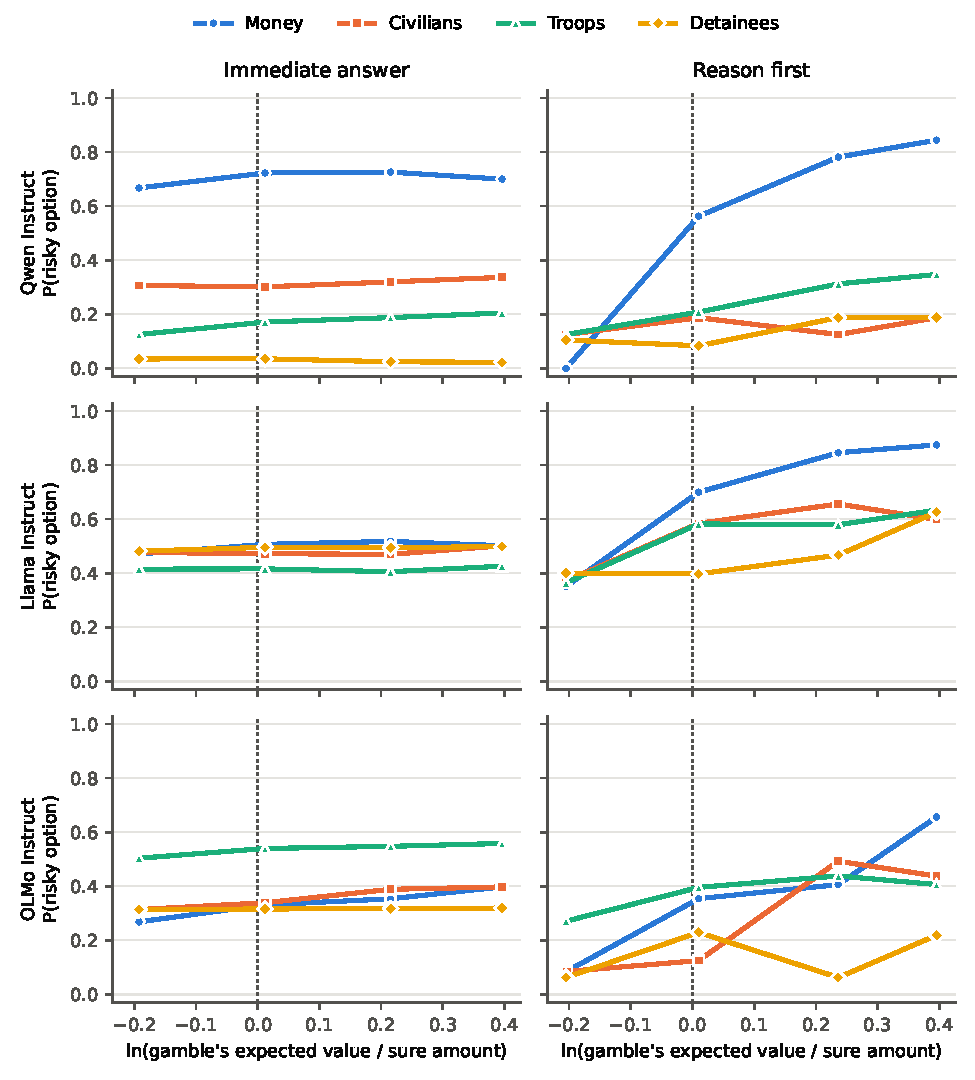
\includegraphics[width=0.72\textwidth,height=\textheight]{figures/fig1_money_vs_lives.pdf}
\caption{Open models. P(risky) against the gamble's expected value
relative to the sure option, money versus lives.}
\end{figure}

\hypertarget{role-matters-less-than-domain}{%
\subsubsection{Role matters less than
domain}\label{role-matters-less-than-domain}}

Deciding rather than recommending changes Qwen's P(risky) by 0.01 to
0.05 within the lives domains, and OLMo's similarly little.

\hypertarget{frontier-models-in-three-modes}{%
\subsection{5. Frontier models in three
modes}\label{frontier-models-in-three-modes}}

All four Claude models engaged with every question. Every free-outcome
control in every domain, mode and wording was answered for the larger
amount (1.00 throughout). Almost every answer parsed. The exception is
Sonnet's snap answers on troops, where 8\% of questions were excluded
for too few usable answers, and every other domain and mode lost 3\% or
less, most of them none. Table 2 gives the main results at low effort,
and Figure 2 plots the shifts.

\emph{Table 2. Shift in P(risky) from money/self {[}95\% CI{]} and
cell-level r with money/self for the Claude models on the main grid,
with roles pooled. ``EV'' is agreement with expected value on clear
questions, and ``tokens'' is mean output tokens per answer, including
the visible answer.}

\begin{longtable}[]{@{}
  >{\raggedright\arraybackslash}p{(\columnwidth - 10\tabcolsep) * \real{0.1667}}
  >{\raggedright\arraybackslash}p{(\columnwidth - 10\tabcolsep) * \real{0.1667}}
  >{\raggedright\arraybackslash}p{(\columnwidth - 10\tabcolsep) * \real{0.1667}}
  >{\raggedright\arraybackslash}p{(\columnwidth - 10\tabcolsep) * \real{0.1667}}
  >{\raggedright\arraybackslash}p{(\columnwidth - 10\tabcolsep) * \real{0.1667}}
  >{\raggedright\arraybackslash}p{(\columnwidth - 10\tabcolsep) * \real{0.1667}}@{}}
\toprule\noalign{}
\begin{minipage}[b]{\linewidth}\raggedright
Model, mode
\end{minipage} & \begin{minipage}[b]{\linewidth}\raggedright
Money P(risky) / EV
\end{minipage} & \begin{minipage}[b]{\linewidth}\raggedright
Civilians
\end{minipage} & \begin{minipage}[b]{\linewidth}\raggedright
Troops
\end{minipage} & \begin{minipage}[b]{\linewidth}\raggedright
Detainees
\end{minipage} & \begin{minipage}[b]{\linewidth}\raggedright
Tokens
\end{minipage} \\
\midrule\noalign{}
\endhead
\bottomrule\noalign{}
\endlastfoot
Sonnet, snap & 1.00 / 0.68 & -0.24 {[}-0.28, -0.19{]}, r 0.27 & -0.23
{[}-0.27, -0.19{]}, r 0.22 & -0.63 {[}-0.69, -0.58{]}, r 0.12 &
\textasciitilde13 \\
Sonnet, written reasoning & 0.47 / 0.99 & -0.23 {[}-0.36, -0.11{]}, r
0.66 & -0.28 {[}-0.43, -0.14{]}, r 0.61 & -0.44 {[}-0.63, -0.25{]}, r
0.27 & 250 \\
Sonnet, extended thinking & 0.54 / 0.98 & -0.26 {[}-0.41, -0.12{]}, r
0.60 & -0.25 {[}-0.40, -0.13{]}, r 0.66 & -0.47 {[}-0.65, -0.29{]}, r
0.29 & 72 \\
Fable, extended thinking & 0.44 / 0.92 & -0.23 {[}-0.32, -0.14{]}, r
0.68 & -0.23 {[}-0.34, -0.12{]}, r 0.69 & -0.38 {[}-0.53, -0.24{]}, r
0.42 & 34 \\
Haiku, snap & 0.51 / 0.55 & -0.09 {[}-0.15, -0.04{]}, r 0.15 & +0.12
{[}0.07, 0.17{]}, r -0.49 & -0.37 {[}-0.42, -0.33{]}, r 0.27 &
\textasciitilde4 \\
Haiku, written reasoning & 0.43 / 0.88 & -0.28 {[}-0.40, -0.17{]}, r
0.66 & -0.23 {[}-0.36, -0.12{]}, r 0.60 & -0.45 {[}-0.61, -0.28{]}, r
0.42 & 244 \\
Haiku, extended thinking & 0.48 / 0.92 & +0.01 {[}-0.03, 0.05{]}, r 0.95
& +0.04 {[}0.02, 0.08{]}, r 0.94 & -0.01 {[}-0.05, 0.02{]}, r 0.94 &
87 \\
Opus, extended thinking & 0.45 / 0.98 & +0.05 {[}-0.00, 0.12{]}, r 0.92
& +0.03 {[}-0.00, 0.07{]}, r 0.93 & -0.06 {[}-0.14, -0.01{]}, r 0.93 &
55 \\
Opus, ext. thinking + written & 0.44 / 0.98 & +0.03 {[}-0.00, 0.07{]}, r
0.94 & +0.00 {[}-0.01, 0.01{]}, r 0.98 & -0.14 {[}-0.25, -0.05{]}, r
0.84 & 304 \\
\end{longtable}

Snap token counts are per-cell totals over five samples divided by five,
rounded, and include little beyond the answer. Source is
\texttt{results/paper\_frontier\_tables.csv}.

\begin{figure}
\centering
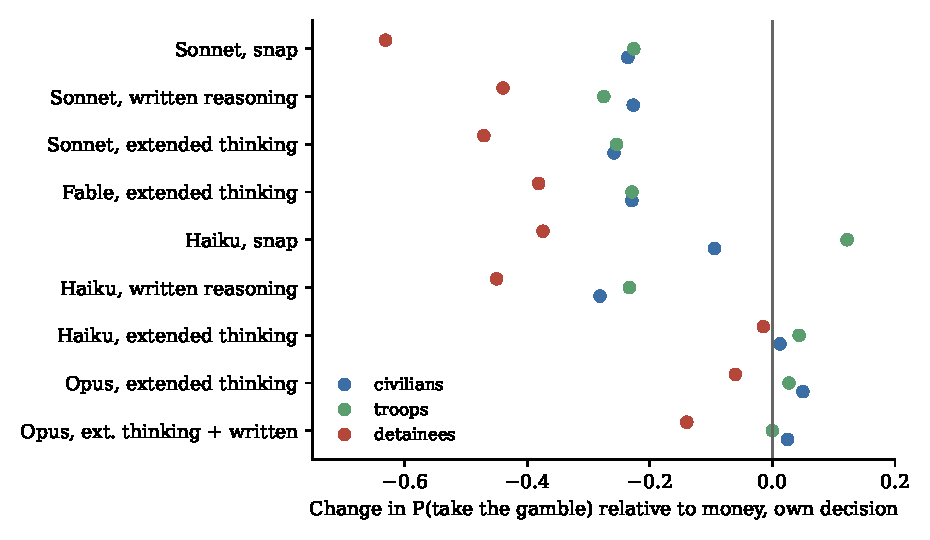
\includegraphics[width=0.85\textwidth,height=\textheight]{figures/fig2_frontier_shift.pdf}
\caption{Shift in the probability of choosing the gamble, lives relative
to money, for each Claude model and mode (low effort, main grid). Zero
means the model treats lives exactly as it treats money.}
\end{figure}

\hypertarget{snap-answers-repeat-the-open-model-result}{%
\subsubsection{Snap answers repeat the open-model
result}\label{snap-answers-repeat-the-open-model-result}}

Sonnet's one-letter answers take the money gamble almost every time. Its
P(risky) is 1.00, and because it takes the gamble even when the gamble
is worth less, its expected-value agreement is only 0.68. With lives at
stake it becomes far more cautious. It is 0.24 less likely to gamble for
civilians, 0.23 less for soldiers and 0.63 less for detained aid
workers, with every interval far from zero. The money answers barely
predict the lives answers (r 0.12 to 0.27). As with Llama, the format of
the question moves Sonnet's snap answers on lives. Listing the gamble
first raises P(risky) by 0.40 for civilians and 0.46 for soldiers,
against 0.01 for money. Haiku's snap answers are erratic in a different
way. The frame sets its money answers, with P(risky) 0.75 lower in the
mixed wording than in the gain wording, and its troop answers run
opposite to its money answers (r = -0.49).

\hypertarget{written-reasoning-makes-the-answers-more-orderly-and-keeps-the-caution}{%
\subsubsection{Written reasoning makes the answers more orderly and
keeps the
caution}\label{written-reasoning-makes-the-answers-more-orderly-and-keeps-the-caution}}

When Sonnet and Haiku reason in the reply before answering, they agree
with expected value on money almost perfectly (0.99 and 0.88). Their
money answers now predict which lives questions draw more risk
moderately well, with r of 0.60 to 0.66 for civilians and soldiers. The
level still differs. Both models remain 0.23 to 0.28 less likely to
gamble for civilians and soldiers and 0.44 to 0.45 less likely for
detainees. The open models' reasoned answers look the same, with Qwen
computing expected value for money and then arguing for certainty with
lives.

\hypertarget{extended-thinking-splits-the-models}{%
\subsubsection{Extended thinking splits the
models}\label{extended-thinking-splits-the-models}}

With extended thinking at low effort, Haiku and Opus treat every domain
like money. Their shifts are within 0.06 of zero, their expected-value
agreement is 0.94 to 1.00 in every domain, and the money answers predict
the lives answers with r of 0.92 to 0.95. Sonnet and Fable behave as
they do without it. With extended thinking they look like Sonnet's
written reasoning, 0.23 to 0.26 more cautious with civilians and
soldiers and 0.38 to 0.47 more cautious with detainees.

\hypertarget{the-length-of-the-reasoning-does-not-explain-the-split}{%
\subsubsection{The length of the reasoning does not explain the
split}\label{the-length-of-the-reasoning-does-not-explain-the-split}}

Haiku's written reasoning runs to about 244 output tokens per answer and
keeps the full gap. Its extended thinking runs to about 87 tokens,
answer included, and closes the gap. Opus closes it in about 55. More
computation on the question therefore cannot account for the change. The
extended-thinking mode itself appears to change which rule the model
applies, and it does so differently in different models. We state the
result accordingly as ``the thinking setting changes the answer''. Opus
cannot turn thinking off, so for Opus the model and the mode cannot be
separated. Haiku can, which makes it the clean case.

\hypertarget{what-this-means-for-screening}{%
\subsubsection{What this means for
screening}\label{what-this-means-for-screening}}

For Haiku and Opus with extended thinking, a money lottery would be a
good screen, since it predicts both the level and the ordering of the
lives answers. In every other case we ran it would get the level wrong
by 0.2 to 0.6 and the ordering only partly right. That covers snap
answers and written reasoning in every model, and Sonnet and Fable in
every mode we tried at low effort. The same Claude model can fall in
either group depending on a setting a user may never see.

\hypertarget{the-second-wording}{%
\subsubsection{The second wording}\label{the-second-wording}}

Stage A2 repeats the grid with independently written templates, and
Table 4 in section 7 gives its detainee rows. The pattern holds. In snap
answers Sonnet is 0.38 to 0.56 more cautious in every lives domain, the
money answers predict nothing (r 0.02 to 0.12), and order effects reach
+0.57. With written reasoning or extended thinking Sonnet stays 0.22 to
0.32 more cautious for civilians and soldiers. Haiku's snap answers are
again driven by the frame, with a money frame gap of -0.90. With
extended thinking, Haiku and Opus stay within 0.05 of money for
civilians and soldiers (r 0.88 to 0.98). One result is weaker in the
second wording. Fable's caution with civilians and soldiers shrinks from
0.23 to 0.11-0.14, though the intervals still exclude zero.

\hypertarget{the-effort-setting-acts-like-a-dose}{%
\subsection{6. The effort setting acts like a
dose}\label{the-effort-setting-acts-like-a-dose}}

Sonnet and Fable let us vary extended-thinking effort within one model.
Table 3 and Figure 3 give the results, with Haiku and Opus shown for
comparison.

\emph{Table 3. Shift in P(risky) from money/self {[}95\% CI{]} by effort
setting, with extended thinking on the main grid. Each row's shift is
measured against the model's own money answers at the same effort.}

\begin{longtable}[]{@{}
  >{\raggedright\arraybackslash}p{(\columnwidth - 12\tabcolsep) * \real{0.1429}}
  >{\raggedright\arraybackslash}p{(\columnwidth - 12\tabcolsep) * \real{0.1429}}
  >{\raggedright\arraybackslash}p{(\columnwidth - 12\tabcolsep) * \real{0.1429}}
  >{\raggedright\arraybackslash}p{(\columnwidth - 12\tabcolsep) * \real{0.1429}}
  >{\raggedright\arraybackslash}p{(\columnwidth - 12\tabcolsep) * \real{0.1429}}
  >{\raggedright\arraybackslash}p{(\columnwidth - 12\tabcolsep) * \real{0.1429}}
  >{\raggedright\arraybackslash}p{(\columnwidth - 12\tabcolsep) * \real{0.1429}}@{}}
\toprule\noalign{}
\begin{minipage}[b]{\linewidth}\raggedright
Model
\end{minipage} & \begin{minipage}[b]{\linewidth}\raggedright
Effort
\end{minipage} & \begin{minipage}[b]{\linewidth}\raggedright
Civilians
\end{minipage} & \begin{minipage}[b]{\linewidth}\raggedright
Troops
\end{minipage} & \begin{minipage}[b]{\linewidth}\raggedright
Detainees
\end{minipage} & \begin{minipage}[b]{\linewidth}\raggedright
r (civ. / troops / det.)
\end{minipage} & \begin{minipage}[b]{\linewidth}\raggedright
Tokens
\end{minipage} \\
\midrule\noalign{}
\endhead
\bottomrule\noalign{}
\endlastfoot
Sonnet & low & -0.26 {[}-0.41, -0.12{]} & -0.25 {[}-0.40, -0.13{]} &
-0.47 {[}-0.65, -0.29{]} & 0.60 / 0.66 / 0.29 & 72 \\
Sonnet & medium & -0.24 {[}-0.39, -0.10{]} & -0.23 {[}-0.38, -0.11{]} &
-0.47 {[}-0.66, -0.29{]} & 0.64 / 0.69 / 0.28 & 73 \\
Sonnet & high & -0.12 {[}-0.20, -0.05{]} & -0.10 {[}-0.19, -0.02{]} &
-0.39 {[}-0.58, -0.22{]} & 0.84 / 0.85 / 0.43 & 90 \\
Fable & low & -0.23 {[}-0.32, -0.14{]} & -0.23 {[}-0.34, -0.12{]} &
-0.38 {[}-0.53, -0.24{]} & 0.68 / 0.69 / 0.42 & 34 \\
Fable & high & -0.12 {[}-0.20, -0.04{]} & -0.04 {[}-0.13, 0.05{]} &
-0.31 {[}-0.45, -0.18{]} & 0.82 / 0.77 / 0.53 & 79 \\
Haiku & low & +0.01 {[}-0.03, 0.05{]} & +0.04 {[}0.02, 0.08{]} & -0.01
{[}-0.05, 0.02{]} & 0.95 / 0.94 / 0.94 & 87 \\
Haiku & high & -0.01 {[}-0.04, 0.01{]} & -0.00 {[}-0.02, 0.01{]} & -0.03
{[}-0.06, 0.00{]} & 0.96 / 0.98 / 0.97 & 138 \\
Opus & low & +0.05 {[}-0.00, 0.12{]} & +0.03 {[}-0.00, 0.07{]} & -0.06
{[}-0.14, -0.01{]} & 0.92 / 0.93 / 0.93 & 55 \\
Opus & high & +0.05 {[}0.01, 0.11{]} & +0.04 {[}0.00, 0.08{]} & -0.07
{[}-0.15, -0.01{]} & 0.92 / 0.93 / 0.90 & 82 \\
\end{longtable}

\begin{figure}
\centering
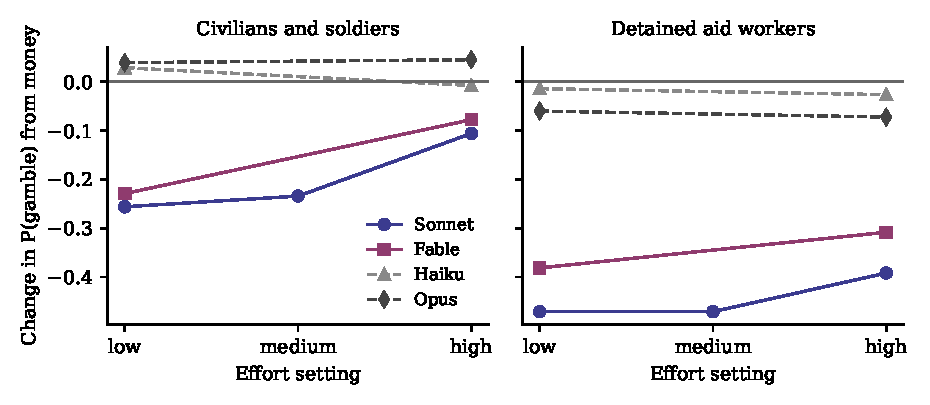
\includegraphics[width=0.85\textwidth,height=\textheight]{figures/fig3_effort_dose.pdf}
\caption{Shift from money by effort setting. The left panel averages
civilians and soldiers and the right panel shows detained aid workers.
Sonnet and Fable move toward money-like choices at high effort for
civilians and soldiers, but not for detainees. Haiku and Opus sit near
zero throughout.}
\end{figure}

\hypertarget{the-response-is-a-step}{%
\subsubsection{The response is a step}\label{the-response-is-a-step}}

Sonnet's answers barely change from low to medium effort, and its
thinking does not lengthen either (72 to 73 tokens). At high effort its
caution with civilians and soldiers halves, from about -0.25 to -0.10 or
-0.12. The money answers then predict the lives answers much better,
with r rising from 0.60-0.69 to 0.84-0.85, and agreement with expected
value on those questions rises from about 0.80 to 0.95-0.97. Fable moves
the same way. Its caution with soldiers almost disappears at high effort
(-0.04, with an interval that includes zero), and its caution with
civilians halves.

\hypertarget{the-change-is-large-relative-to-the-extra-thinking}{%
\subsubsection{The change is large relative to the extra
thinking}\label{the-change-is-large-relative-to-the-extra-thinking}}

Sonnet's high-effort answers use about 18 more tokens than its
low-effort answers, and Fable's about 45 more. Thinking at these
settings is short in absolute terms, and no model averaged more than 140
output tokens per answer in any extended-thinking run. These data cannot
say whether the change comes from the content of the extra tokens or
from a broader effect of the setting on the model's policy. They do show
that the setting, which a deployer chooses and a user typically does not
see, changes the answer to a lives question by as much as the difference
between two models.

\hypertarget{detainees-barely-move}{%
\subsubsection{Detainees barely move}\label{detainees-barely-move}}

At high effort Sonnet is still 0.39 less likely to gamble for detained
aid workers than for money, and Fable 0.31 less likely. The money
answers still explain little of the detainee answers (r 0.43 and 0.53).
Effort closes most of the gap for civilians and soldiers and little of
it for detainees. Section 7 takes up why.

\hypertarget{the-detainee-exception}{%
\subsection{7. The detainee exception}\label{the-detainee-exception}}

The detainee domain draws the most caution in every open model and in
every Claude mode except extended thinking in Haiku and Opus. The
detainee question differs from the others in two ways. The people at
stake are hostages in a negotiation rather than people to be moved, and
the failure branch in the original wording adds that ``the crisis
escalates''. The release variant removes the escalation clause and keeps
everything else.

\emph{Table 4. Shift in P(risky) from money/self {[}95\% CI{]} for
detainees in the second wording and for the release variant (the
original wording without escalation), Stage A2, low effort.}

\begin{longtable}[]{@{}
  >{\raggedright\arraybackslash}p{(\columnwidth - 4\tabcolsep) * \real{0.3333}}
  >{\raggedright\arraybackslash}p{(\columnwidth - 4\tabcolsep) * \real{0.3333}}
  >{\raggedright\arraybackslash}p{(\columnwidth - 4\tabcolsep) * \real{0.3333}}@{}}
\toprule\noalign{}
\begin{minipage}[b]{\linewidth}\raggedright
Model, mode
\end{minipage} & \begin{minipage}[b]{\linewidth}\raggedright
Detainees, second wording
\end{minipage} & \begin{minipage}[b]{\linewidth}\raggedright
Release, no escalation
\end{minipage} \\
\midrule\noalign{}
\endhead
\bottomrule\noalign{}
\endlastfoot
Sonnet, snap & -0.41 {[}-0.46, -0.37{]} & -0.54 {[}-0.60, -0.48{]} \\
Sonnet, written reasoning & -0.45 {[}-0.65, -0.25{]} & -0.40 {[}-0.58,
-0.23{]} \\
Sonnet, extended thinking & -0.46 {[}-0.62, -0.31{]} & -0.43 {[}-0.58,
-0.29{]} \\
Fable, extended thinking & -0.34 {[}-0.48, -0.19{]} & -0.29 {[}-0.41,
-0.18{]} \\
Haiku, snap & -0.42 {[}-0.44, -0.39{]} & -0.31 {[}-0.35, -0.28{]} \\
Haiku, written reasoning & -0.41 {[}-0.56, -0.25{]} & -0.40 {[}-0.55,
-0.25{]} \\
Haiku, extended thinking & -0.10 {[}-0.17, -0.03{]} & -0.04 {[}-0.07,
-0.01{]} \\
Opus, extended thinking & -0.10 {[}-0.20, -0.04{]} & -0.04 {[}-0.10,
0.00{]} \\
\end{longtable}

\begin{figure}
\centering
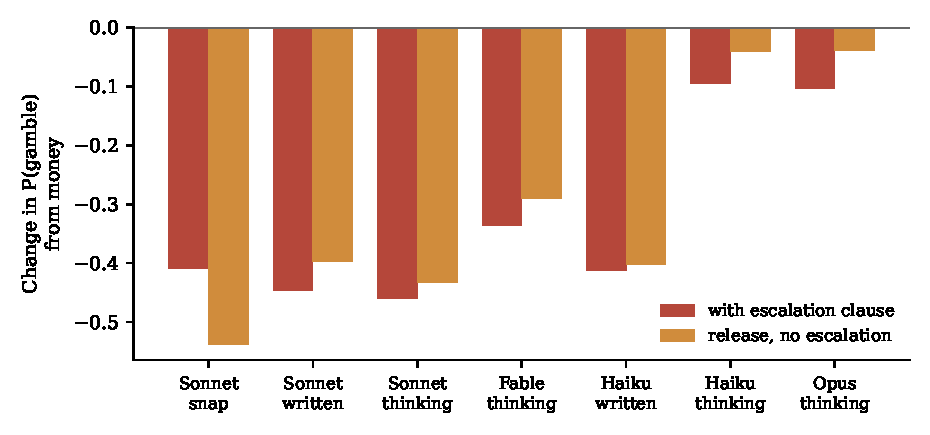
\includegraphics[width=0.85\textwidth,height=\textheight]{figures/fig4_release.pdf}
\caption{Caution about detainees with and without the escalation clause
(second-wording run). Removing escalation leaves the caution almost
unchanged in every model and mode that shows it.}
\end{figure}

\hypertarget{the-caution-holds-across-wordings}{%
\subsubsection{The caution holds across
wordings}\label{the-caution-holds-across-wordings}}

The second, independently written detainee template produces shifts of
-0.34 to -0.46 for Sonnet, Fable and Haiku without extended thinking,
close to the original wording's -0.38 to -0.63.

\hypertarget{the-models-cite-escalation-and-escalation-does-not-drive-the-choice}{%
\subsubsection{The models cite escalation, and escalation does not drive
the
choice}\label{the-models-cite-escalation-and-escalation-does-not-drive-the-choice}}

Sonnet's written reasoning on the original detainee questions mentions
escalation in every answer. About 60\% of answers call the outcome
irreversible, and about 75\% refer to the detainees who would remain or
to later talks. Escalation never comes up for civilians or soldiers. Yet
deleting the escalation clause changes almost nothing. Sonnet with
written reasoning or extended thinking is 0.40 to 0.43 more cautious in
the release variant, against 0.45 to 0.46 for the second-wording
detainee questions and 0.44 to 0.47 in the main grid. Fable is 0.29 more
cautious against 0.34, and Haiku with written reasoning 0.40 against
0.41. In snap answers Sonnet is, if anything, more cautious without
escalation (-0.54). This is a clear behavioral case of a stated
rationale that does not track the decision, in line with work on the
faithfulness of model explanations (Samway et al.~2025).

\hypertarget{what-does-drive-it}{%
\subsubsection{What does drive it}\label{what-does-drive-it}}

The data narrow the candidates without settling the question. The
caution is specific to a sure release offered in a negotiation. It is
larger than for civilians or soldiers facing the same numbers, it barely
responds to effort, and it is insensitive to the expected value of the
gamble. Sonnet's expected-value agreement on detainees stays at 0.54 to
0.62 at every effort, near what a model would score by mostly declining
the gamble. Three accounts fit these facts.

\begin{enumerate}
\def\labelenumi{\arabic{enumi}.}
\tightlist
\item
  \emph{A protected value.} Turning down a deal that frees people for
  certain, in order to gamble on freeing more, resembles the trade-offs
  people treat as taboo (Tetlock 2003). Protected values are insensitive
  to quantity and resist reflection (Baron and Spranca 1997), which fits
  a caution that survives effort and ignores expected value.
\item
  \emph{Act versus accept.} Pressing for full release is an act that
  puts the sure group at risk, while accepting the deal is the default.
  Language models show a stronger omission bias than people (Cheung,
  Maier and Lieder 2025).
\item
  \emph{Learned negotiation norms.} Hostage-negotiation guidance often
  favors securing the release on offer, and a model could carry that as
  learned content rather than as a value.
\end{enumerate}

A variant in which the sure outcome requires the action and the gamble
is the default would separate the first account from the second. We
leave it for future work.

\hypertarget{the-exception-belongs-to-some-models-only}{%
\subsubsection{The exception belongs to some models
only}\label{the-exception-belongs-to-some-models-only}}

With extended thinking, Haiku and Opus treat detainees nearly like
money, at -0.04 to -0.10 in Stage A2 and -0.01 to -0.07 in the main
grid. Opus is slightly the more cautious of the two, and its residual
detainee caution grows when it also writes out its reasoning (-0.14),
but the effect is small beside Sonnet's and Fable's.

\hypertarget{why-lottery-answers-transfer-poorly}{%
\subsection{8. Why lottery answers transfer
poorly}\label{why-lottery-answers-transfer-poorly}}

The project's earlier phases, run on the same 40 gambles, help explain
why a lottery measurement carries over to lives so unevenly.

\hypertarget{framing-tracks-the-stated-gain}{%
\subsubsection{Framing tracks the stated
gain}\label{framing-tracks-the-stated-gain}}

When the model of gain-versus-loss wording includes a constant term, the
loss-aversion estimate is close to zero, and the gap between gain and
loss wording follows the size of the stated gain
(\texttt{notes/phase3-robustness-2026-10-03.md}). The models do not
apply a stable value function with a kink at a reference point. They
respond to how the question is worded, and that sensitivity carries over
unevenly to lives. Qwen's frame gap is +0.50 to +0.62 for civilians and
absent for detainees, and Haiku's snap money answers are driven almost
entirely by the frame, with gaps of -0.75 and -0.90 in the two wordings.
A risk attitude that depends on wording in money will not transfer
cleanly to a domain with different wording.

\hypertarget{rules-bind-only-when-the-model-reasons}{%
\subsubsection{Rules bind only when the model
reasons}\label{rules-bind-only-when-the-model-reasons}}

When told to maximize expected value, the open models comply 0.80 to
0.97 of the time if they reason first and near chance in one-letter
answers, across paraphrases of the rule
(\texttt{docs/robustness-results-2026-10-03.md}, PR \#1). Snap answers
are the less controllable regime, which fits the format effects in
Llama's and Sonnet's snap answers on lives. The frontier results refine
this. Reasoning is necessary for a consistent rule, and it is not
sufficient. Sonnet and Haiku with written reasoning apply expected value
to money and still decline it for lives, and only some models in the
extended-thinking mode apply it everywhere.

\hypertarget{leftover-biases-are-model-specific}{%
\subsubsection{Leftover biases are
model-specific}\label{leftover-biases-are-model-specific}}

Stating the rule and requiring reasoning raises agreement between models
from 0.52 to 0.84, but the remaining frame gap differs in sign across
models (\texttt{notes/convergence-question-2026-10-05.md}). The Claude
results show the same thing at the level of the domain gap. Four models
from one developer split into two groups, and the split depends on the
mode. There is no single ``LLM risk attitude'' to measure once and apply
everywhere.

\hypertarget{implications-for-evaluating-advisory-ai}{%
\subsection{9. Implications for evaluating advisory
AI}\label{implications-for-evaluating-advisory-ai}}

\hypertarget{the-thinking-setting-is-part-of-the-model}{%
\subsubsection{The thinking setting is part of the
model}\label{the-thinking-setting-is-part-of-the-model}}

The same Claude model can give opposite recommendations on a lives
question depending on the extended-thinking mode and effort. Sonnet's
caution with civilians halves between medium and high effort. A risk
evaluation run at one setting therefore does not carry to a deployment
at another. Evaluations of risk posture, and of values more generally,
should report the mode and effort the way a clinical trial reports the
dose, and should be run at the setting used in deployment.

\hypertarget{lottery-screening-is-conditional-and-the-lottery-does-not-reveal-the-condition}{%
\subsubsection{Lottery screening is conditional, and the lottery does
not reveal the
condition}\label{lottery-screening-is-conditional-and-the-lottery-does-not-reveal-the-condition}}

A money lottery predicts lives advice well for Opus and for Haiku with
extended thinking, with r of about 0.9 and a shift near zero. It
predicts poorly for snap answers, for written reasoning, and for Sonnet
and Fable at the settings we tried. An evaluator would have to run the
advisory questions to learn which case applies, and at that point the
lottery adds little. The general claim of the paper therefore holds in a
sharper form. Risk attitudes for advisory use have to be measured on
advisory questions, in the domain of use, at the deployed setting.

\hypertarget{quick-use-and-planning-use-may-get-different-advisers}{%
\subsubsection{Quick use and planning use may get different
advisers}\label{quick-use-and-planning-use-may-get-different-advisers}}

A quick-turn tool that runs with thinking off gets the cautious,
human-like answer, with a strong pull from option order. A planning cell
running at high effort gets something closer to an expected-value
calculator for civilians and soldiers, and still a cautious negotiator
for detainees. Neither is labeled as such, and a user comparing the two
would see the same model name.

\hypertarget{neither-posture-is-clearly-correct}{%
\subsubsection{Neither posture is clearly
correct}\label{neither-posture-is-clearly-correct}}

Choosing by expected lives saved is the impartial answer, and much
planning doctrine leans that way. Many human decision-makers might
prefer the certain partial outcome, and people trust advisers who resist
cold trade-offs (Everett, Pizarro and Crockett 2016). We do not claim
that the thinking modes are more rational or better with lives, and the
data cannot settle whether expected value is the right rule for lives.
Our point is that the posture should be known, measured on the right
questions, and disclosed.

\hypertarget{stated-reasons-can-mislead}{%
\subsubsection{Stated reasons can
mislead}\label{stated-reasons-can-mislead}}

In the detainee questions Sonnet cites escalation in every answer, yet
removing escalation does not change its choice. A commander reading the
rationale would learn the wrong thing about why the model said no.
Evaluators can test a stated rationale by removing the element it cites,
as the release variant does, and checking whether the choice moves.

\hypertarget{practical-recommendations}{%
\subsubsection{Practical
recommendations}\label{practical-recommendations}}

We suggest four practices for evaluators. Test advisory risk posture on
advisory questions in the domain of use. Report snap, written-reasoning
and extended-thinking answers separately, together with the effort
setting. Include free-outcome controls and both option orders, since
snap answers on lives can be set by order. Check that the model's stated
reason drives its choice by removing that reason from the question.

\hypertarget{limitations}{%
\subsection{10. Limitations}\label{limitations}}

The thinking in these runs is short. Even at high effort, no model
averaged more than about 140 output tokens per answer with extended
thinking. The finding is that the effort setting changes the answer, and
we make no claim about long reasoning. Haiku and Opus close the gap with
almost no thinking, which points to a change in policy rather than a
computation, but our data cannot tell the two apart.

Model and mode are entangled for Opus and Fable, since neither can run
with thinking off, so their behavior with thinking cannot be compared
with their behavior without it. Haiku and Sonnet, which were run in all
modes, and the effort ladders within Sonnet and Fable are the clean
within-model tests.

All the frontier results come from four Claude models, which share a
developer and much of a training lineage. The open models reproduce the
snap and written-reasoning pattern, but the extended-thinking results
have no outside replication. The most useful next step would be a model
from another developer with an adjustable thinking setting.

Claude P(risky) values come from three or five sampled answers per
question at the default temperature, so individual values are coarse.
Gamble-cluster intervals account for this in the averages. Sampling
noise attenuates the correlations with money, so the r values for the
frontier models are lower bounds on the underlying agreement. The
open-model values are exact probabilities, with greedy reasoning and a
single seed.

The second wording reproduces the main pattern, but Fable's caution with
civilians and soldiers is about half as large in it. Results for
individual domains other than detainees should be read as moderately
sensitive to wording. The open models were run on one wording per
domain, and the second wording and release variant on the Claude models
only.

The stakes are hypothetical and the vignettes are short. Real decisions
involve uncertainty about the numbers themselves, more context, and
dialogue. Stage B of this project, with realistic scenarios, has not yet
been run.

There is no human baseline on these items, so comparisons with people
rest on other studies' tasks. A small survey on the same items, under
time pressure and with required justification, would show whether snap
answers or thinking answers are closer to human advisers.

Finally, OLMo was prompted few-shot with money exemplars. The detainee
domain bundles hostages with negotiation, and the act-versus-accept
variant described in section 7 is untested. Model behavior may change in
future versions of the same models, and all Claude runs were made in
October 2026.

\hypertarget{conclusion}{%
\subsection{11. Conclusion}\label{conclusion}}

We asked whether a language model's risk attitude, measured on money
lotteries, predicts its advice when lives are at stake. For open models,
and for frontier models answering quickly or reasoning in writing, it
does not. These models become much more cautious with lives, by amounts
the money answers do not reveal, and their quick advice on lives can be
set by the order of the options. With extended thinking, two of four
Claude models choose by expected value in every domain and the lottery
becomes a good predictor. In the other two, more effort moves the
answers toward the money pattern for civilians and soldiers but not for
detained aid workers, whose caution survives every setting and wording
we tried, as well as the removal of the reason the models give for it. A
model's risk posture over lives is a property of the model together with
its thinking setting. Evaluations meant to tell deployers how a model
will advise should be run on advisory questions at the setting used in
deployment, and should say which setting that was.

\hypertarget{references}{%
\subsection{References}\label{references}}

{[}All entries to be checked against the original sources before arXiv.
Entries marked * were found in the October 2026 literature search and
have not yet been checked in full.{]}

\begin{itemize}
\tightlist
\item
  Bago, B., and De Neys, W. (2019). The intuitive greater good: Testing
  the corrective dual process model of moral cognition. \emph{Journal of
  Experimental Psychology: General}, 148(10).
\item
  Baron, J., and Spranca, M. (1997). Protected values.
  \emph{Organizational Behavior and Human Decision Processes}, 70(1),
  1-16.
\item
  Bini, S., Cong, L. W., Huang, D., and Jin, L. (2026). Behavioral
  economics of AI: LLM biases and corrections. NBER Working Paper 34745.
  arXiv:2602.09362.
\item
  Binz, M., and Schulz, E. (2023). Using cognitive psychology to
  understand GPT-3. \emph{PNAS}, 120(6), e2218523120.
\item
  Chen, Y., Liu, T. X., Shan, Y., and Zhong, S. (2023). The emergence of
  economic rationality of GPT. \emph{PNAS}, 120(51), e2316205120.
\item
  Cheung, V., Maier, M., and Lieder, F. (2025). Large language models
  show amplified cognitive biases in moral decision-making. \emph{PNAS}.
  doi:10.1073/pnas.2412015122.*
\item
  Everett, J. A. C., Pizarro, D. A., and Crockett, M. J. (2016).
  Inference of trustworthiness from intuitive moral judgments.
  \emph{Journal of Experimental Psychology: General}, 145(6), 772-787.
\item
  Fagley, N. S., and Miller, P. M. (1997). Framing effects and arenas of
  choice: Your money or your life? \emph{Organizational Behavior and
  Human Decision Processes}, 71(3), 355-373.
\item
  Gema, A. P., et al.~(2025). Inverse scaling in test-time compute.
  arXiv:2507.14417.*
\item
  Greene, J. D., Sommerville, R. B., Nystrom, L. E., Darley, J. M., and
  Cohen, J. D. (2001). An fMRI investigation of emotional engagement in
  moral judgment. \emph{Science}, 293(5537), 2105-2108.
\item
  Greene, J. D., Morelli, S. A., Lowenberg, K., Nystrom, L. E., and
  Cohen, J. D. (2008). Cognitive load selectively interferes with
  utilitarian moral judgment. \emph{Cognition}, 107(3), 1144-1154.
\item
  Hagendorff, T., Fabi, S., and Kosinski, M. (2023). Human-like
  intuitive behavior and reasoning biases emerged in large language
  models but disappeared in ChatGPT. \emph{Nature Computational
  Science}, 3, 833-838.
\item
  Himmelreich, J. (2026). {[}Replication of Pfeffer, Krügel and Uhl
  2025.{]} arXiv:2603.22730.*
\item
  Holt, C. A., and Laury, S. K. (2002). Risk aversion and incentive
  effects. \emph{American Economic Review}, 92(5), 1644-1655.
\item
  Horton, J. J. (2023). Large language models as simulated economic
  agents: What can we learn from homo silicus? NBER Working Paper 31122.
\item
  Hosseini, {[}initials{]}, Khanna, {[}initials{]}, and Pierce,
  {[}initials{]} (2026). The judgment-consequence gap.
  arXiv:2608.05583.*
\item
  Itzhak, I., Stanovsky, G., Rosenfeld, N., and Belinkov, Y. (2024).
  Instructed to bias: Instruction-tuned language models exhibit emergent
  cognitive bias. \emph{Transactions of the ACL}, 12.
\item
  Lamparth, M., Corso, A., Ganz, J., Mastro, O. S., Schneider, J., and
  Trinkunas, H. (2024). Human vs.~machine: Behavioral differences
  between expert humans and language models in wargame simulations.
  \emph{Proceedings of AIES 2024}.
\item
  LeBoeuf, R. A., and Shafir, E. (2003). Deep thoughts and shallow
  frames: On the susceptibility to framing effects. \emph{Journal of
  Behavioral Decision Making}, 16(2), 77-92.
\item
  Liu, J., Yang, Y., and Tam, K. Y. (2025). Evaluating and aligning
  human economic risk preferences in LLMs. \emph{Proceedings of EMNLP
  2025}. arXiv:2503.06646.
\item
  Mazeika, M., et al.~(2025). Utility engineering: Analyzing and
  controlling emergent value systems in AIs. arXiv:2502.08640.
\item
  Mei, Q., Xie, Y., Yuan, W., and Jackson, M. O. (2024). A Turing test
  of whether AI chatbots are behaviorally similar to humans.
  \emph{PNAS}, 121(9), e2313925121.
\item
  Pfeffer, {[}initials{]}, Krügel, S., and Uhl, M. (2025). {[}Reasoning
  models and utilitarian moral judgment; full reference to add.{]}*
\item
  Raji, I. D., Bender, E. M., Paullada, A., Denton, E., and Hanna, A.
  (2021). AI and the everything in the whole wide world benchmark.
  \emph{NeurIPS Datasets and Benchmarks Track}.
\item
  Rivera, J.-P., Mukobi, G., Reuel, A., Lamparth, M., Smith, C., and
  Schneider, J. (2024). Escalation risks from language models in
  military and diplomatic decision-making. \emph{Proceedings of FAccT
  2024}.
\item
  Röttger, P., Hofmann, V., Pyatkin, V., Hinck, M., Kirk, H. R.,
  Schütze, H., and Hovy, D. (2024). Political compass or spinning arrow?
  Towards more meaningful evaluations for values and opinions in large
  language models. \emph{Proceedings of ACL 2024}.
\item
  Samway, K., et al.~(2025). {[}Chain-of-thought and post-hoc moral
  explanations.{]} \emph{Proceedings of EMNLP 2025}. arXiv:2505.21479.*
\item
  Tetlock, P. E. (2003). Thinking the unthinkable: Sacred values and
  taboo cognitions. \emph{Trends in Cognitive Sciences}, 7(7), 320-324.
\item
  Tetlock, P. E., Kristel, O. V., Elson, S. B., Green, M. C., and
  Lerner, J. S. (2000). The psychology of the unthinkable. \emph{Journal
  of Personality and Social Psychology}, 78(5), 853-870.
\item
  Trhlik, {[}initials{]}, et al.~(2026). LLMs contain multitudes.
  arXiv:2606.13944.*
\item
  Tversky, A., and Kahneman, D. (1981). The framing of decisions and the
  psychology of choice. \emph{Science}, 211(4481), 453-458.
\item
  Wang, Y., Li, X., and Chen, G. (2025). Risk profiling and modulation
  for LLMs. arXiv:2509.23058.
\end{itemize}

\hypertarget{appendix-a.-claude-runs}{%
\subsection{Appendix A. Claude runs}\label{appendix-a.-claude-runs}}

All runs used \texttt{src/api\_elicit.py} against the native Anthropic
API in October 2026, with the models \texttt{claude-haiku-5-5},
\texttt{claude-sonnet-5-5}, \texttt{claude-opus-5-5} and
\texttt{claude-fable-5-1}. Total cost was \$97.92, from the author's
monthly API credits.

\begin{longtable}[]{@{}
  >{\raggedright\arraybackslash}p{(\columnwidth - 6\tabcolsep) * \real{0.2500}}
  >{\raggedright\arraybackslash}p{(\columnwidth - 6\tabcolsep) * \real{0.2500}}
  >{\raggedright\arraybackslash}p{(\columnwidth - 6\tabcolsep) * \real{0.2500}}
  >{\raggedright\arraybackslash}p{(\columnwidth - 6\tabcolsep) * \real{0.2500}}@{}}
\toprule\noalign{}
\begin{minipage}[b]{\linewidth}\raggedright
Run
\end{minipage} & \begin{minipage}[b]{\linewidth}\raggedright
Questions
\end{minipage} & \begin{minipage}[b]{\linewidth}\raggedright
Samples each
\end{minipage} & \begin{minipage}[b]{\linewidth}\raggedright
Cost (USD)
\end{minipage} \\
\midrule\noalign{}
\endhead
\bottomrule\noalign{}
\endlastfoot
Haiku, snap / written reasoning / thinking low / thinking high & 1,440 /
800 / 800 / 800 & 5 / 3 / 3 / 3 & 0.10 / 0.33 / 0.13 / 0.19 \\
Haiku, second wording, snap / written / thinking low & 1,800 / 1,000 /
1,000 & 5 / 3 / 3 & 0.13 / 0.47 / 0.20 \\
Sonnet, snap / written reasoning / thinking low & 1,440 / 800 / 800 & 5
/ 3 / 3 & 2.66 / 6.69 / 2.31 \\
Sonnet, thinking medium / thinking high & 800 / 800 & 3 / 3 & 2.34 /
2.74 \\
Sonnet, second wording, snap / written / thinking low & 1,800 / 1,000 /
1,000 & 5 / 3 / 3 & 3.43 / 9.05 / 3.26 \\
Opus, thinking low / thinking + written / thinking high & 800 / 800 /
800 & 3 / 3 / 3 & 3.82 / 15.99 / 5.10 \\
Opus, second wording, thinking low & 1,000 & 3 & 5.14 \\
Fable, thinking low / thinking high & 800 / 800 & 3 / 3 & 7.02 /
12.58 \\
Fable, second wording, thinking low & 1,000 & 3 & 8.95 \\
\end{longtable}

The remainder of the total went to pilots, a high-effort test slice and
probes. {[}Recompute the table with \texttt{python\ scripts/spend.py}
before arXiv. The Sonnet second-wording reasoning run was completed in
two parts (\$7.41 and \$1.64).{]}

\hypertarget{appendix-b.-reproducing-the-numbers}{%
\subsection{Appendix B. Reproducing the
numbers}\label{appendix-b.-reproducing-the-numbers}}

\begin{itemize}
\tightlist
\item
  Open models use \texttt{python\ analysis/stage\_a.py} and
  \texttt{python\ analysis/stage\_a\_bounds.py}.
\item
  Claude models use \texttt{python\ analysis/paper\_frontier\_tables.py}
  (writes \texttt{results/paper\_frontier\_tables.csv}), or
  \texttt{python\ analysis/stage\_a.py\ -\/-stems\ \textless{}stems\textgreater{}}
  for the per-role tables.
\item
  Figure 1 comes from \texttt{python\ analysis/make\_paper\_figures.py}
  and Figures 2-4 from
  \texttt{python\ analysis/make\_frontier\_figures.py}.
\item
  The data are in \texttt{data/stageA\_*.csv} (main grid) and
  \texttt{data/stageA\_*\_a2*.csv} (second wording and release).
\end{itemize}

\end{document}
